\section{Stati Coerenti}

Gli stati coerenti forniscono una descrizione classica della luce in termini di onde elettromagnetiche, nonostante siano stati costruiti a partire dalla meccanica quantistica. Solitamente, vengono rappresentati come $|\alpha_j \rangle = |q_j + ip_j \rangle $, utilizzando la notazione introdotta da Paul Dirac, nota come notazione "bra-ket". Da notare che uno stato coerente è caratterizzato da due componenti, \textit{q} e \textit{p}, chiamate componenti di quadratura, che non hanno un valore esatto, ma sono variabili aleatorie che seguono una distribuzione di probabilità gaussiana. In opportune unità di misura, questa distribuzione ha una varianza unitaria. La ragione per cui non rappresentano un valore esatto è dovuta al fatto che, in fisica quantistica, anche le quantità scalari sono operatori che assumono un valore esatto solo al momento della misura.

Il numero medio di fotoni in uno stato coerente può essere calcolato nel seguente modo:
\begin{equation}
\langle n_j \rangle = |a_j|^2 = q^2 + p^2
\end{equation}

Il numero medio di fotoni in uno stato coerente è correlato all'energia del segnale di luce trasmesso: maggiore è il numero di fotoni, maggiore è l'energia del segnale.

Come accennato in precedenza, gli stati coerenti nel nostro contesto si presentano come una distribuzione di probabilità gaussiana e possono essere rappresentati graficamente nel piano di Gauss come una nuvola di punti, ognuno dei quali segue una distribuzione gaussiana.

\begin{figure}[tbp]
\begin{center}
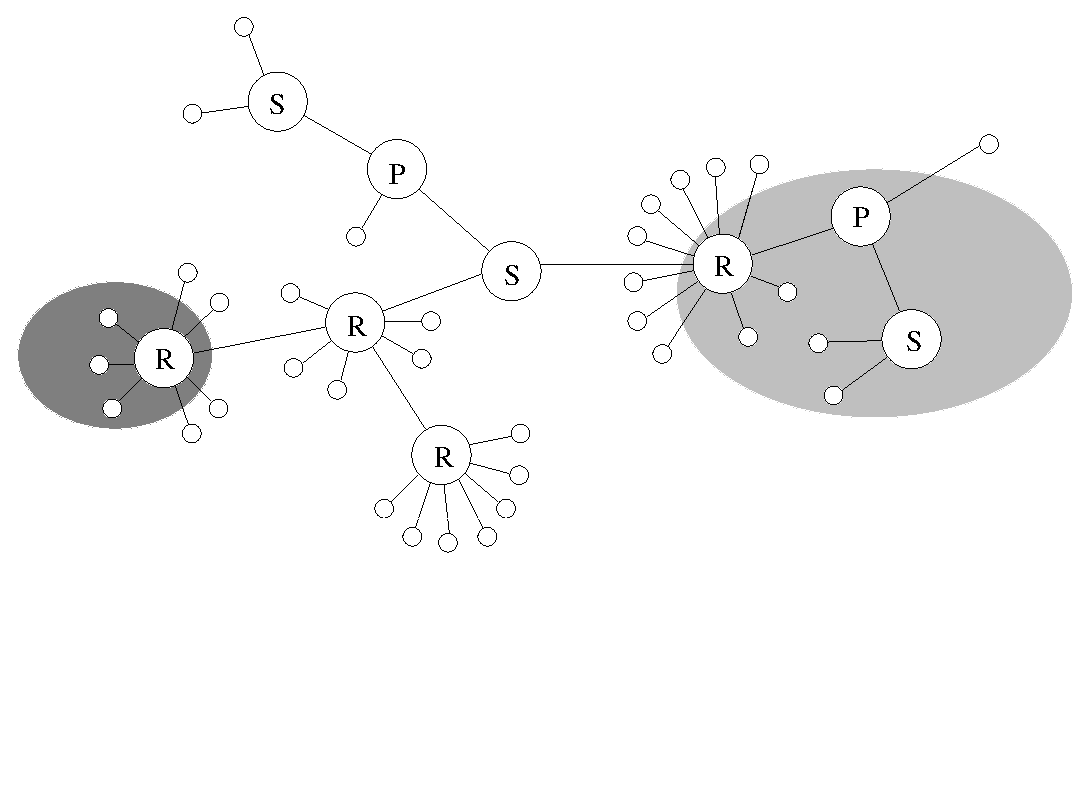
\includegraphics[width=8cm]{figure/esempio-figura-1.eps}
\end{center}
\caption{Esempio di rappresentazione grafica degli stati coerenti} \label{fig:stato-coerente}
\end{figure}

\section{Comportamento durante la Misura}

Durante la fase di misura, Bob riceve uno stato coerente con la forma illustrata nella figura \ref{fig:stato-coerente}. È da aspettarsi che, al momento della ricezione, il valore della deviazione standard delle gaussiane che descrivono lo stato coerente aumenti rispetto a quello che aveva durante la fase di trasmissione. Questo aumento dell'incertezza è dovuto al rumore introdotto dal canale di trasmissione, ma ne discuteremo dettagliatamente nel capitolo \ref{cap:capitolo_2}.

Una volta ricevuto il segnale quantistico, Bob effettua una misura che comporta l'estrazione, in base al tipo di misura, di uno o due valori con una distribuzione gaussiana. Dopo questa fase di misura, si conclude la parte quantistica del protocollo, e si ottengono dati classici su cui verranno eseguite ulteriori operazioni per determinare se è possibile stabilire una chiave di crittografia sicura o se è necessario abortire la trasmissione e iniziare nuovamente da capo.